\documentclass{beamer}

\mode<presentation>
{
  \usetheme{Berkeley}
  \usecolortheme{seagull}
  \setbeamercovered{transparent}
}

\title{Nuclear Engineering}
\author{Jeffrey Seifried}
\institute{Ad Delivery Team, Yelp}
\date{Advanced Learning Group, \texttt{2015-03-16}}

\AtBeginSubsection[]
{
  \begin{frame}<beamer>{Outline}
    \tableofcontents[currentsection,currentsubsection]
  \end{frame}
}


\begin{document}

\begin{frame}
  \titlepage
\end{frame}

\begin{frame}{Outline}
  \tableofcontents
\end{frame}


\section{About Me}

    \begin{frame}{I've studied Nuclear Engineering for over a decade}{...and all I got was this stupid tshirt}

        \begin{itemize}

            \item BS at University of Maryland, College Park
            \begin{itemize}
                \item Became a nuclear reactor operator
            \end{itemize}

            \pause

            \item PhD at UC, Berkeley and Lawrence Livermore Lab
            \begin{itemize}
                \item Developed reactor simulations
                \item Propagated uncertainties through them
                \item Helped design a hybrid fusion-fission reactor
            \end{itemize}

            \pause

            \item postdoc
            \begin{itemize}
                \item Developed reactor simulations
                \item Taught a course on nuclear reactor physics
                \item Helped design a thorium-fueled breed and burn reactor
            \end{itemize}
        \end{itemize}

    \end{frame}

\section{Nuclear Energy}

\subsection{The state of the neutron}

    \begin{frame}{Nuclear energy is important for electricity production in the US}

        \begin{columns}[T]

            \begin{column}{0.5\textwidth}
                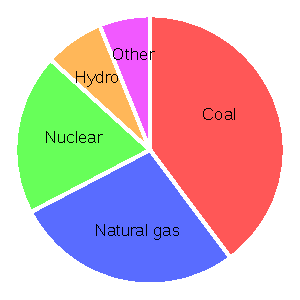
\includegraphics{./img/sources.pdf}
            \end{column}

            \begin{column}{0.5\textwidth}
                \begin{itemize}
                    \item Nuclear power generates 20\% of all electricity
                    \pause
                    \item ...and 60\% of carbon-free electricity
                    \pause
                    \item The most recent plant was built in 1996
                    \pause
                    \item ...its construction began in 1978
                    \pause
                    \item Fossil Fuels generate 66\%
                    \pause
                    \item Renewables are ``other''
                \end{itemize}
            \end{column}

        \end{columns}

    \end{frame}

    \begin{frame}{Energy production has a real world impact}

        \begin{itemize}
            \item Coal causes 10 thousand deaths annually in the US
            \pause
            \item One quarter of California air pollution is from China
            \pause
            \item Climate change is just starting
            \pause
            \item Natural gas and oil just got a lot cheaper
        \end{itemize}

    \end{frame}

\subsection{We've come a long way since 1978}

    \begin{frame}{Fast reactors}
    \end{frame}

    \begin{frame}{Fluoride-salt-cooled high-temperature reactors}
    \end{frame}

    \begin{frame}{Breed and burn reactors}
    \end{frame}

    \begin{frame}{Hybrid fusion-fission reactors}
    \end{frame}

\section{Simulations}

\subsection{Solving the neutron transport equation}

    \begin{frame}{The neutron transport equation}
    \end{frame}

\subsection{Solving the Bateman equations}

    \begin{frame}{The Bateman equations}
    \end{frame}

\section*{Summary}

    \begin{frame}{Summary}

    \end{frame}

\end{document}
